\documentclass[a4paper,12pt]{article}
\usepackage{CodeReport}

\begin{document}


\begin{center} % Everything within the center environment is centered.
	{\Large \bf Coding Report 1} % <---- Don't forget to put in the right number
	\vspace{2mm}
	
       
	{\bf January 10, 2023}
\end{center}  

\vspace{0.4cm}


\section{Problem Description}
This report demonstrates 4 different methods of finding root on functions with one variable.
The methods are Bisection, Fixed Point, Newton, and Secant method.
Given a function $f \in C[a, b]$, 
we apply the above 4 methods to approximate a sequence of $p_n$ to the real root $p$.

For each method on each function,
we set the maximum iteration to 15 and threshold to $1 \times 10^{-4}$,
meaning that if
$$
|p_{i+1} - p_{i}| < 1 \times 10^{-4}
$$
we said the algorithm converged and stop iterating.


\begin{figure}[H]
    \centering
	\begin{subfigure}[b]{0.49\textwidth}
	    \centering
	    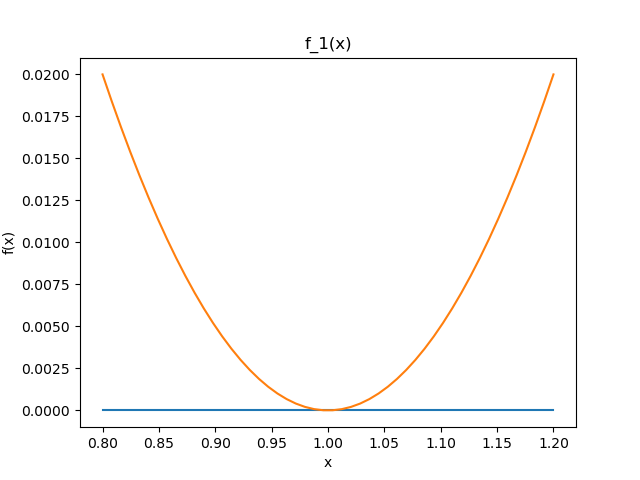
\includegraphics[width=\textwidth]{img/report1/f1.png}
	    \caption{$f_1(x) = \frac{1}{2}\sin((x - 1)^2)$}
	    \label{fig:0}
	\end{subfigure}
	\hfill
	\begin{subfigure}[b]{0.49\textwidth}
	    \centering
	     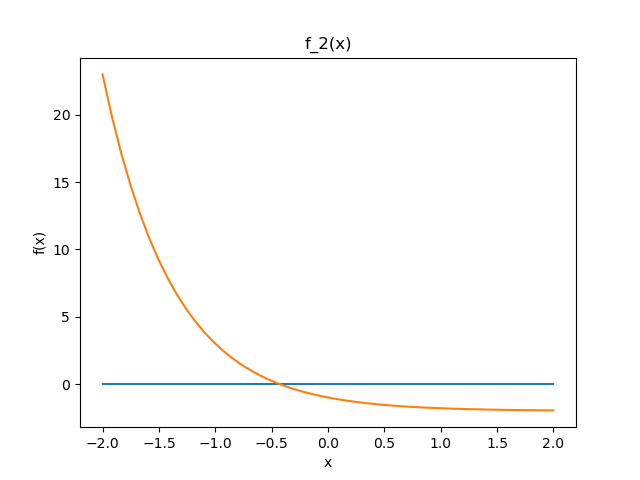
\includegraphics[width=\textwidth]{img/report1/f2.png}
	     \caption{$f_2(x) = 5^{-x} - 2$}
	     \label{fig:1}
	\end{subfigure}
	\caption{Plots showing the true roots of $f_1$ and $f_2$.}
\end{figure}


\section{Results}

\subsection{Root finding results of $f_1$}


Since the graph at Figure 1 (a) shows that the root is in $[0.8, 1.2]$,
we chose $[0.8, 1]$ as the interval for Bisection method,
and 0.8, and (0.8, 0.9) as initial guess for Newton's method and Secant method.
For Fixed Point method, we did a little transformation of the original function,
let
$$
\begin{aligned}
f_{1}(x) & = \frac{1}{2}\sin((x - 1)^2) = 0 \\
\implies & \sin((x - 1)^2) = 0 \\
\implies & (x - 1)^2 = \arcsin(0) \\
\implies & x = \sqrt{\arcsin(0)} + 1 = g_1(x)
\end{aligned}
$$
and then chose 3 as the initial $p$, which is just a random guess.

\begin{table}
\begin{center}
	\begin{tabular}{lrrrr}
	\toprule
	{} &  Bisection &  Fixed\_Point &    Newton &    Secant \\
	\midrule
	0  &   0.100000 &          2.0 &  0.200000 &  0.200000 \\
	1  &   0.050000 &          0.0 &  0.099947 &  0.100000 \\
	2  &   0.025000 &          0.0 &  0.049972 &  0.066656 \\
	3  &   0.012500 &          0.0 &  0.024986 &  0.039995 \\
	4  &   0.006250 &          0.0 &  0.012493 &  0.024997 \\
	5  &   0.003125 &          0.0 &  0.006246 &  0.015383 \\
	6  &   0.001563 &          0.0 &  0.003123 &  0.009523 \\
	7  &   0.000781 &          0.0 &  0.001562 &  0.005882 \\
	8  &   0.000391 &          0.0 &  0.000781 &  0.003636 \\
	9  &   0.000195 &          0.0 &  0.000390 &  0.002247 \\
	10 &   0.000098 &          0.0 &  0.000195 &  0.001389 \\
	11 &   0.000098 &          0.0 &  0.000098 &  0.000858 \\
	12 &   0.000098 &          0.0 &  0.000098 &  0.000530 \\
	13 &   0.000098 &          0.0 &  0.000098 &  0.000328 \\
	14 &   0.000098 &          0.0 &  0.000098 &  0.000203 \\
	\bottomrule
	\end{tabular}
	\caption{Absolute Errors of $p_n$ when approximating root of $f_1$}
\end{center}
\end{table}

\begin{figure}[H]
    \centering
     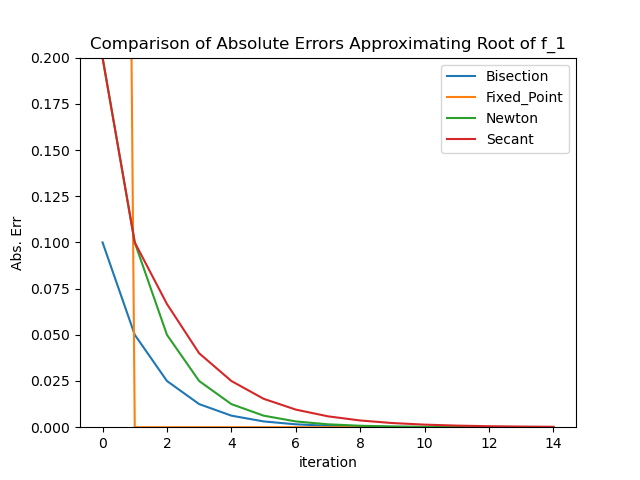
\includegraphics[width=0.8\textwidth]{img/report1/f1_err.png}
     \caption{Absolute Error of each methods approximating $f_1$ with respect to iteration.}
     \label{fig:2}   
\end{figure}

\subsection{Root finding results of $f_2$}

We chose (-2, 2) as interval for Bisection method since the true root is around 0.5.
The the initial guess for Newton's and Secant method,
-2 and (-2, -1),
are taken from ke lower end of the interval.
For Fixed Point method, we just used the default transformation
$$
g_2(x) = x - f_2(x)
$$
but made the initial guess at $-0.43066$ or otherwise the algorithm will not converge.

\begin{table}[H]
\begin{center}
	\begin{tabular}{lrrrr}
	\toprule
	{} &  Bisection &  Fixed\_Point &        Newton &        Secant \\
	\midrule
	0  &   0.430677 &     0.000017 &  1.569323e+00 &  1.569323e+00 \\
	1  &   0.569323 &     0.000070 &  9.976953e-01 &  5.693234e-01 \\
	2  &   0.069323 &     0.000070 &  5.010892e-01 &  4.193235e-01 \\
	3  &   0.180677 &     0.000070 &  1.571370e-01 &  1.497136e-01 \\
	4  &   0.055677 &     0.000070 &  1.829585e-02 &  4.345545e-02 \\
	5  &   0.006823 &     0.000070 &  2.667606e-04 &  4.971415e-03 \\
	6  &   0.024427 &     0.000070 &  8.940697e-08 &  1.716018e-04 \\
	7  &   0.008802 &     0.000070 &  2.980232e-08 &  6.854534e-07 \\
	8  &   0.000989 &     0.000070 &  2.980232e-08 &  2.980232e-08 \\
	9  &   0.002917 &     0.000070 &  2.980232e-08 &  2.980232e-08 \\
	10 &   0.000964 &     0.000070 &  2.980232e-08 &  2.980232e-08 \\
	11 &   0.000012 &     0.000070 &  2.980232e-08 &  2.980232e-08 \\
	12 &   0.000476 &     0.000070 &  2.980232e-08 &  2.980232e-08 \\
	13 &   0.000232 &     0.000070 &  2.980232e-08 &  2.980232e-08 \\
	14 &   0.000110 &     0.000070 &  2.980232e-08 &  2.980232e-08 \\
	\bottomrule
	\end{tabular}
	\caption{Absolute Errors of $p_n$ when approximating root of $f_2$}
\end{center}
\end{table}

\begin{figure}[H]
    \centering
     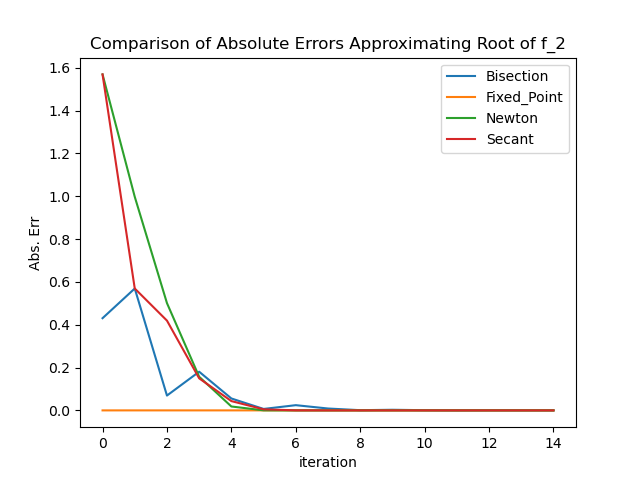
\includegraphics[width=0.8\textwidth]{img/report1/f2_err.png}
     \caption{Absolute Error of each methods approximating $f_2$ with respect to iteration.}
     \label{fig:3}   
\end{figure}





\section{Collaboration}
No collaboration on this project.


\section{Academic Integrity}
On my personal integrity as a student and member of the UCD community, I have not given nor received any unauthorized assistance on this assignment.


\section{Appendix}

\lstinputlisting[language=Python]{numerical_methods/root_finding_1_var.py}
\lstinputlisting[language=Python]{report1.py}

\end{document}